\subsection{Stopped Kaon}
In this section, we compare some quantities of data and MC simulation that K stops in the liquid argon detector and we can find stopped point.
Figure \ref{KsomeQuantities} shows Data and MC comparison for signal hit charge, signal width, decay point and total particle charge distribution.
Data of signal charge and signal width are consistent with MC one in error by less than two $\%$ and data of cluster charge and primary charge are consistent with  MC one in error by less than five $\%$.

Figure \ref{cq27_hough} shows signal hit charge distribution of restricted channel 27. 
As shown in figure \ref{cq27_hough}, signal charge have two peaks at 300 and 500 ADCus.
Because two peaks has correlation of $\Delta$TOF, possible assumption of the cause is that beam line were bipolarrized and the beam didn't pass in the center of the detector.
So, we use only the event that signal charge of restricted channel 27 is less than 350.
Figure \ref{RangeVsHit_hough} shows signal hit charge distribution in different distance from the stopped point.

\begin{figure}[htbp]
  \begin{center}
    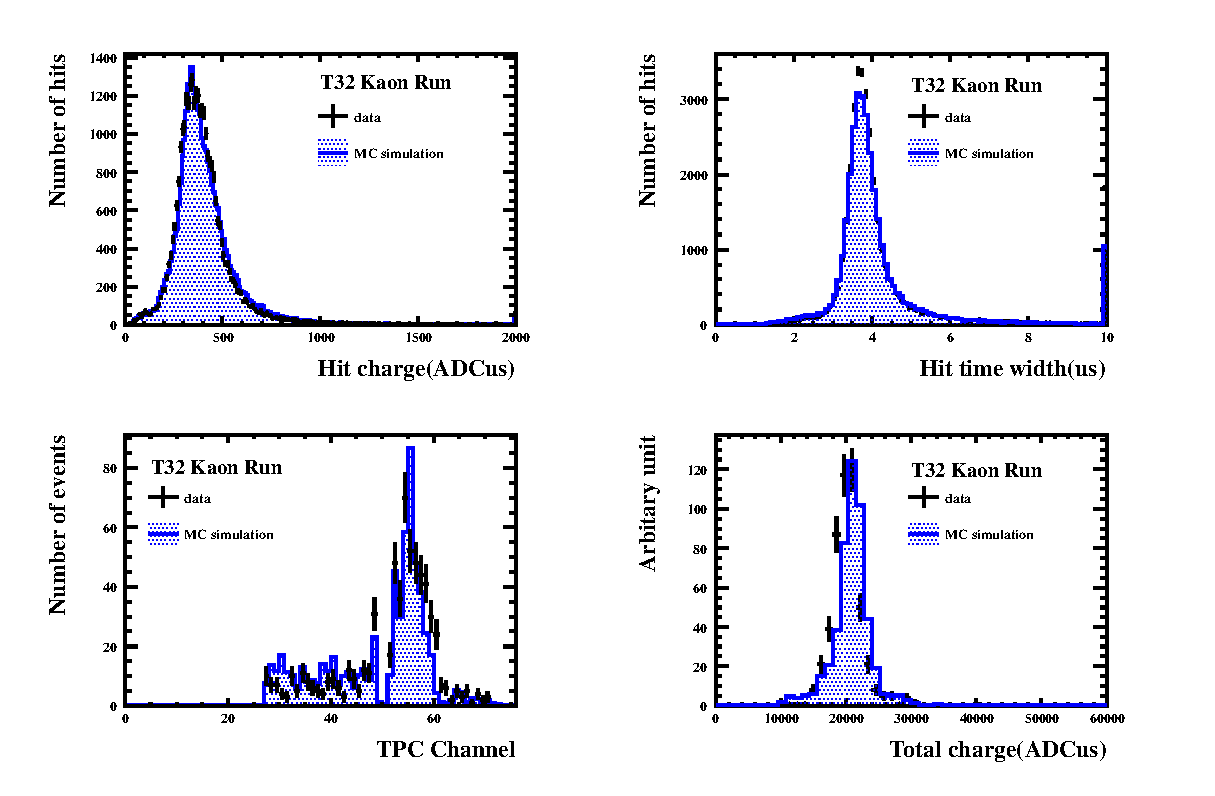
\includegraphics[width=70mm]{fig/cHit4_hough.eps}
  \end{center}    
    \caption{Data-MC comparison for hit charge, hit sigma, cluster charge, primary particle charge}
    \label{KsomeQuantities}
\end{figure}



\begin{figure}[!htb]
  \begin{center}
    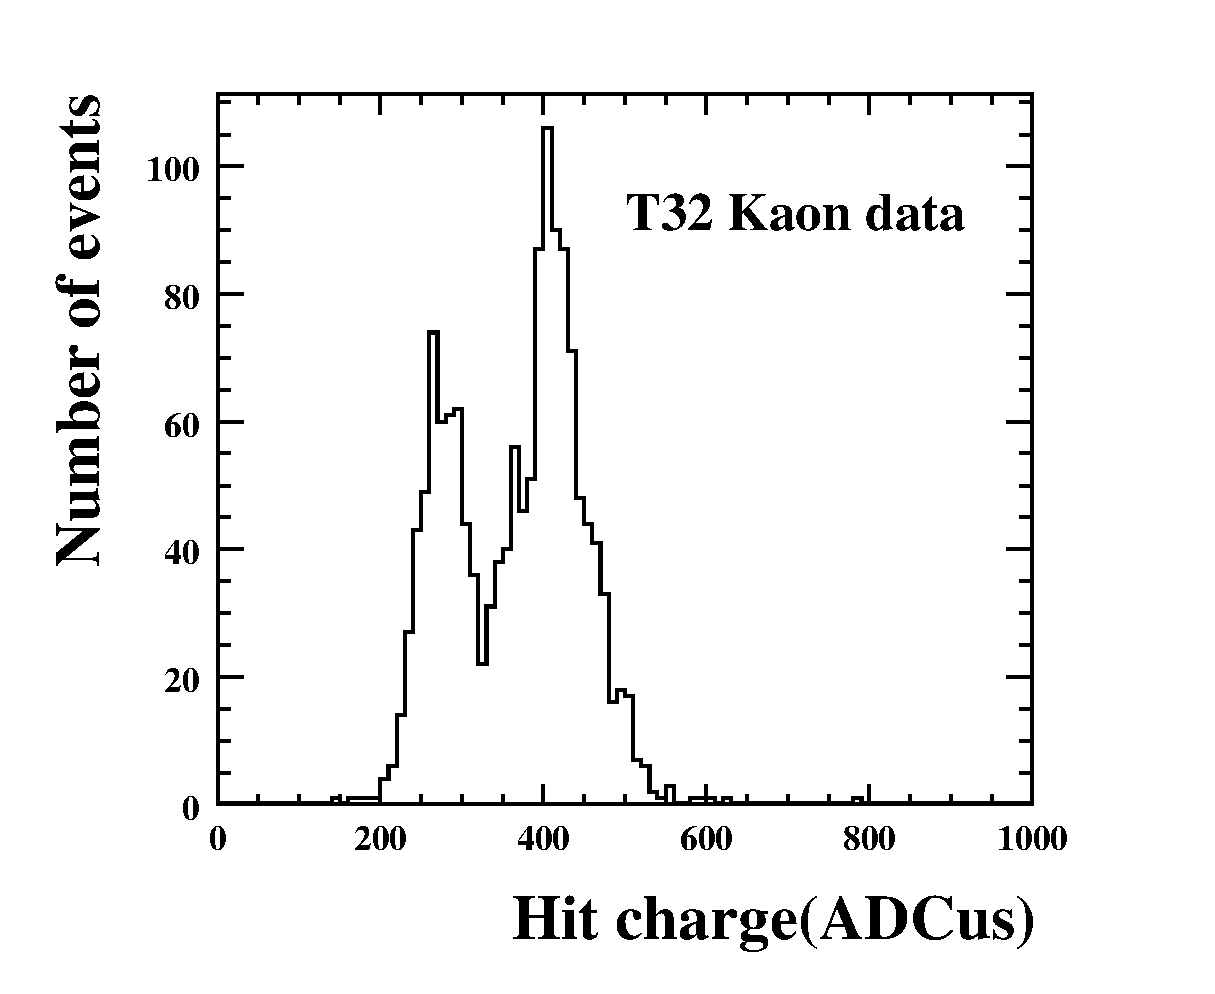
\includegraphics[width=70mm]{fig/ch27distribution.eps}
  \end{center}
  \label{cq27_hough}
  \caption{Hit charge in channel 27}
\end{figure}

\begin{figure}[!htb]
  \begin{center}
    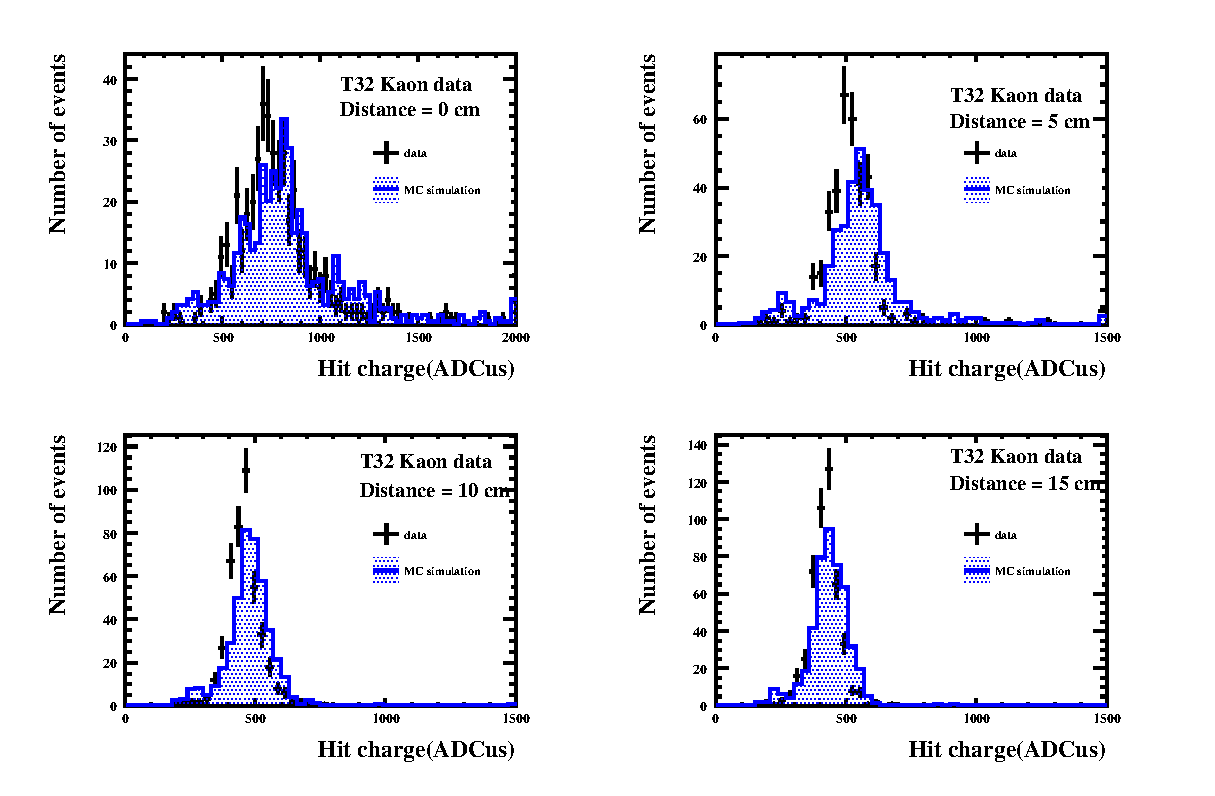
\includegraphics[width=100mm]{fig/RangeVsHit4_wcut_hough.eps}
  \end{center}
  \caption{Data-MC comparison for hit charge distribution in different distance from the stopped point(top left:decay point,top light:decay point-5cm,bottom left:decay point-10cm,decay point-15cm)}
  \label{RangeVsHit_hough}
\end{figure}

As shown in figure \ref{RangeVsHit_hough}, data is consistent with MC one.
Figure \ref{RangeVsHitRatio_hough} shows data/MC ratio of signal hit charge distribution in different distance from the stopped point.
Data of signal charge in different distance from stopped point are consistent with MC one with in 5$\%$.

\begin{figure}[htb]
  \begin{center}
    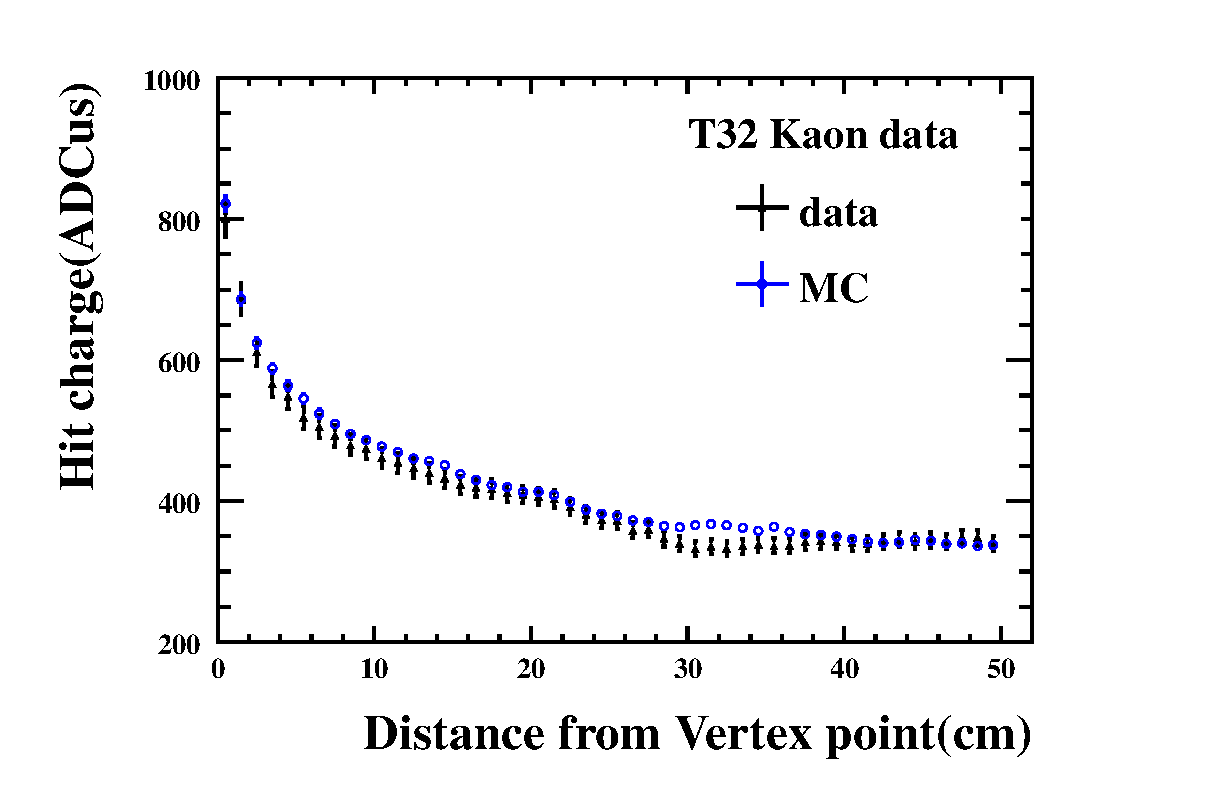
\includegraphics[width=70mm]{fig/RangeVsHitfabs_wcut_hough.eps}
  \end{center}
  \caption{Data-MC comparison for hit charge distribution in different distance from the stopped point}
  \label{RangeVsHitfabs_hough}
\end{figure}

\begin{figure}[htb]
  \begin{center}
    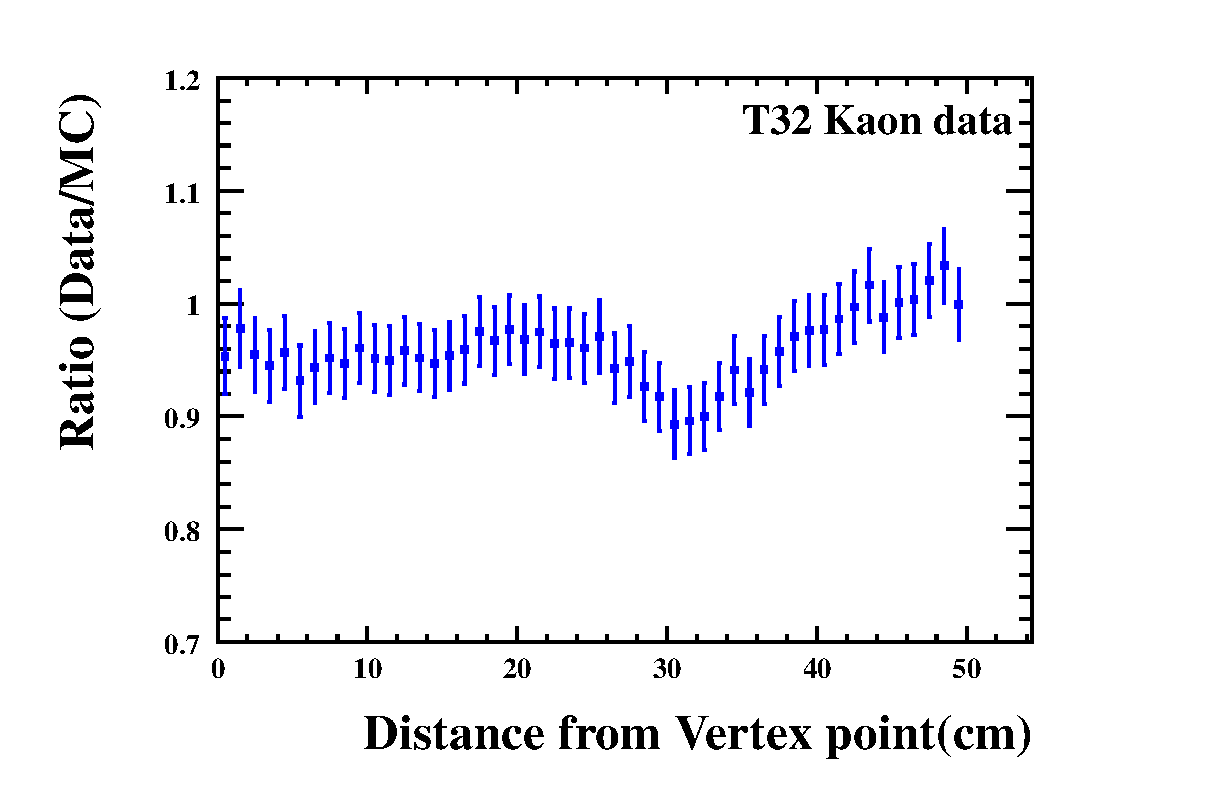
\includegraphics[width=70mm]{fig/RangeVsHitRatio_wcut_hough.eps}
  \end{center}
  \caption{Data/MC ratio for hit charge distribution in different distance from the stopped point}
  \label{RangeVsHitRatio_hough}
\end{figure}



